\section{Network Design}
\label{sec:networkdesign}
In this section, we discuss the problem of how to optimally purchase processing capacity so to satisfy a given flow demand. Although this can be modeled in multiple ways, we limit our discussion to the case where each vertex $v$ has a potential processing capacity $\hat{C}$, which can only be utilized if $\hat{C}$ is purchased.  As in the previous section, this yields two general categories of optimization problems
\begin{enumerate}
	\item The \textit{minimization} version of the problem ({\sc Min Middlebox Purchase}), where the goal is to pick the smallest set of vertices such that all flow is routable.
	\item The \textit{maximization} version of the problem ({\sc Max Middlebox Purchase}), where we try to maximize the amount of routable flow while subject to a budget constraint of $k$. 
\end{enumerate}

Formally, the input to {\sc Min Middlebox Purchase} is a graph $G = (V,E)$ with nonnegative costs $q_v$ on its vertices, a potential processing capacity $C : V \rightarrow \nonnegativereal$, and a collection of $(s_i, t_i)$ pairs with demands $R_i$. The goal is to select a set $T \subseteq V$ of vertices such that all demands are satisfied.  {\sc Max Middlebox Purchase} is given the same collection of inputs along with a budget integer $k$, and the goal is to route as much of the demand as possible.

We begin with the simple observation that {\sc Min Middlebox Purchase} and {\sc Max Middlebox Purchase} inherit the hardness of {\sc Set Cover} and {\sc Max $k$-Coverage}, respectively.

\subsection{Hardness of Network Design}
\begin{figure}[t]
\centering
 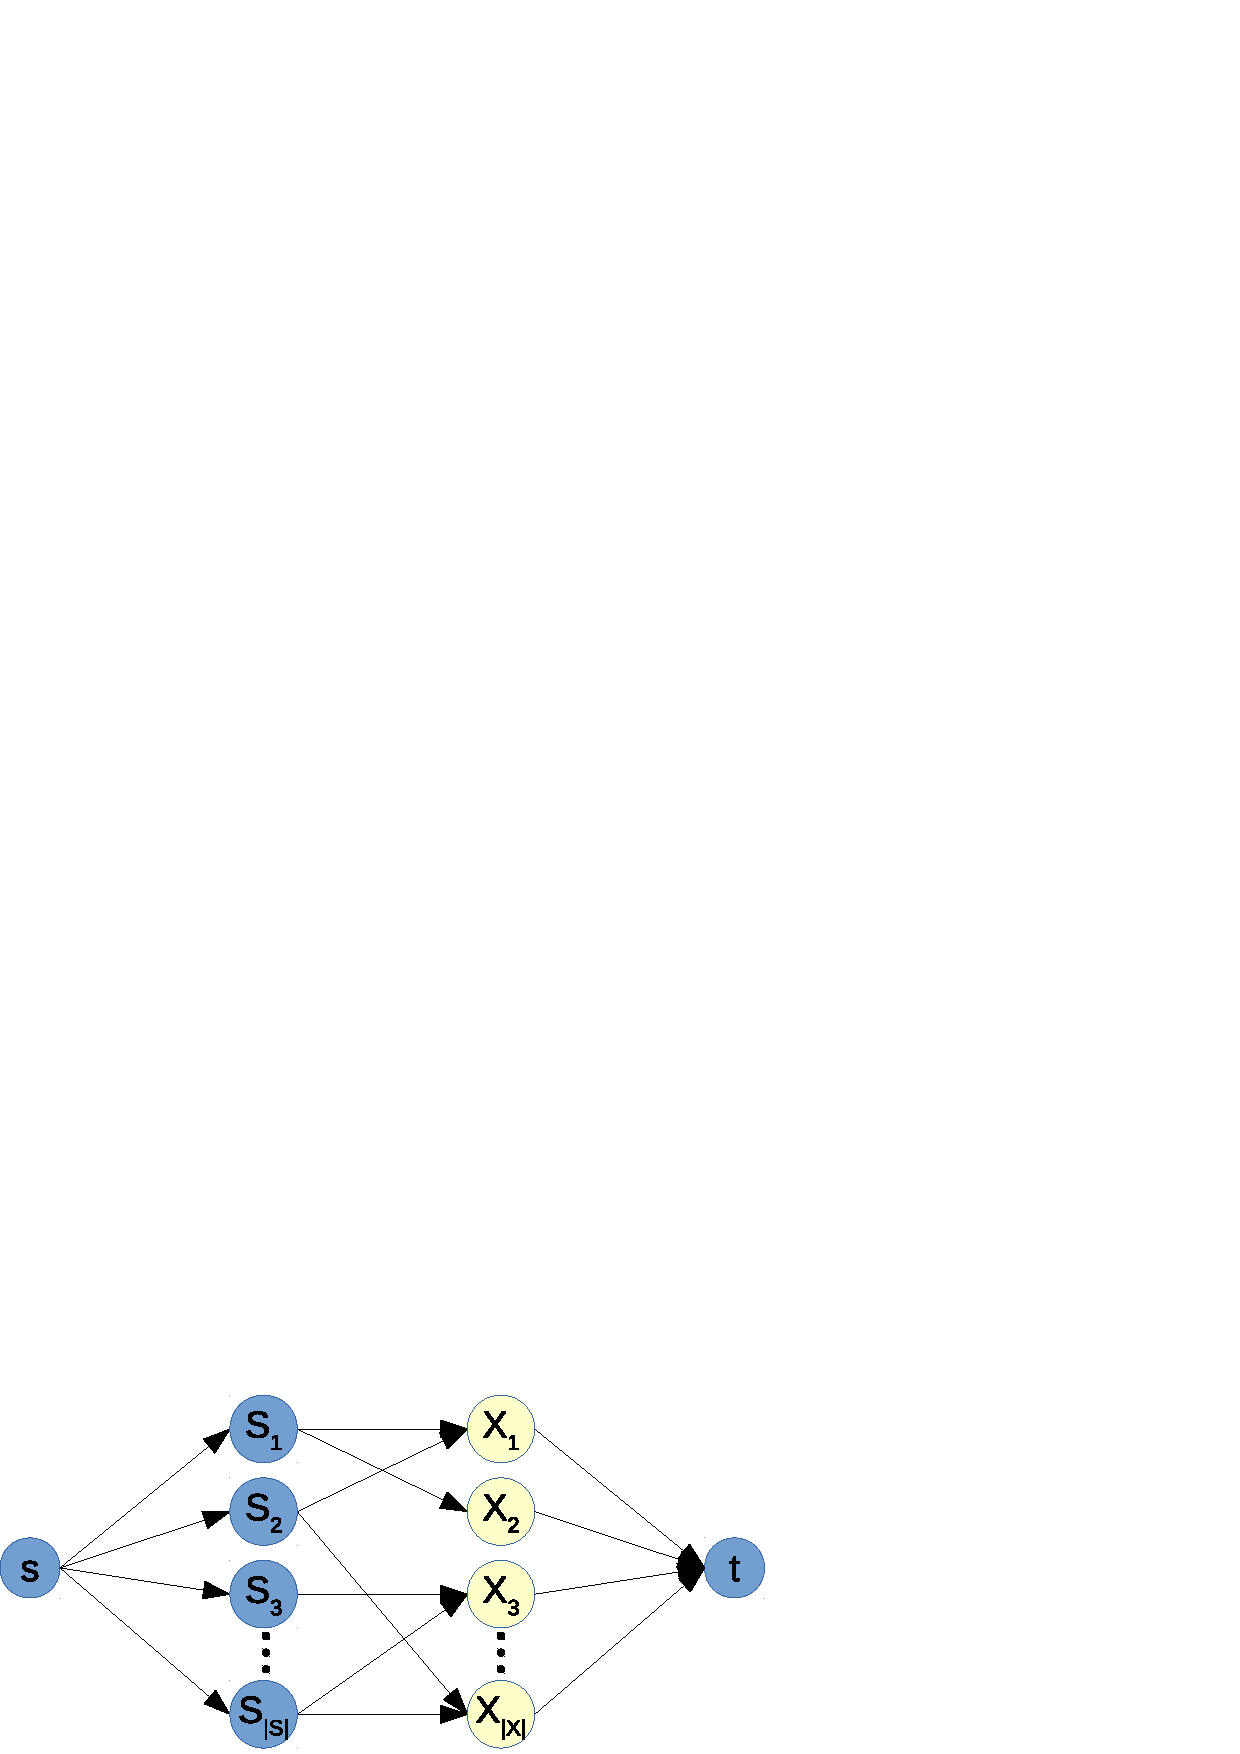
\includegraphics[height=2in]{images/setcover.pdf}
 \caption{Approximation-preserving reduction from {\sc Set Cover} and {\sc Max $k$-Coverage} to {\sc Min Middlebox Purchase} and {\sc Max Middlebox Purchase}. All edges have infinite capacity, blue vertices have $0$ potential capcity, yellow vertices have $|X|$ potential capacity. All purchase costs are 1.}
\label{fig:setcoverreduction}
\end{figure}

\begin{thm}
\label{thm:allocminloghard}
It is $\nph$ to approximate {\sc Min Middlebox Purchase} to within a factor better than $.2267 \log n$. Further, there is no $(1-\epsilon)\log n$-approximation algorithm for {\sc Min Middlebox Purchase} unless $\np \subseteq \dtime(n^{O(\log \log n)})$. These results hold even when the algorithm is allowed to satisfy a mere $\epsilon$-fraction of each demand yet is compared to an exactly-satisfying optimal solution.
\end{thm}

\begin{thm}
\label{thm:allocmaxapxhard}
It is $\nph$ to approximate {\sc Max Middlebox Purchase} to within a factor better than $1 - 1/e$. 
\end{thm}

The reduction for both \Cref{thm:allocminloghard} and \Cref{thm:allocmaxapxhard} is provided in \Cref{fig:setcoverreduction}. In both cases, we create one vertex $S_i$ for each $S$ in the set system $\mathcal{S}$, and one vertex $X_j$ for each $\mathcal{X}$. Each vertex $S_i$ is connected to vertex $X_j$ for each $X_j \in S_i$. Each $S_i$ is given $\mathcal{|X|}$ potential capacity, while all other vertices are given $0$ capacity. Finally, all edges from $X_i$ to $t$ are given capacity $1$, and all other edges are assigned unlimited capacity. Thus, the total amount of flow that can be sent from $s$ to $t$ is exactly the number of vertices $X_j$ connected to $s$ through a purchased vertex $S_i$. It is thus easy to verify that solutions to {\sc Max Middlebox Purchase} and {\sc Min Middlebox Purchase} on this graph exactly correspond to solutions to {\sc Max $k$-Coverage} and {\sc Set Cover}, respectively, which, together with known hardness bounds of those two problems\cite{AMS06}\cite{Feige98}, implies \Cref{thm:allocminloghard} and \Cref{thm:allocmaxapxhard}. Finally, by removing vertex $T$ and setting one unit of flow demand from $S$ to each of the $X_i$, we note that any solution satisfying each demand pair some $\epsilon$ amount is able to satisfy it at equality, as any fractional solution in the above constructions can be rounded up without any loss of feasibility, proving the last statement of \Cref{thm:allocminloghard}.

\begin{figure}[t]
\centering
 \includegraphics[height=1.7in]{images/notsubmodular.pdf}
 \caption{Example graph where vertex purchasing is not submodular. White vertices have no processing potential, colored vertices have 1 potential unit of processing. Solid black edges have capacity $2$ while dashed red edges have capacity $1$. If the only purchased vertex is $r$, no single additional purchase can increase the routable flow at all, yet buying both $u_1$ and $u_2$ simultaneously increases it to $2$.}
\label{fig:notsubmodular}
\end{figure}

It is tempting to state that the amount of routable flow is submodular in the collection of purchased vertices, which would imply that simple greedy algorithms would match the bounds of \Cref{thm:allocminloghard} and \Cref{thm:allocmaxapxhard}. As shown in \Cref{fig:notsubmodular}, this natural supposition happens to be false, as there exist configurations where the natural greedy algorithm gets stuck at an infeasible solution.

\subsection{A bicriterion approximation algorithm}
We describe a modification of the walk based LP formulation with additional 
variables $x_v$ corresponding to whether or not processing capacity at vertex $v$ has been purchased.
We further give a polynomial sized edge-based LP formulation with flow variables $f_i^{1,v}(e)$ and $f_i^{2,v}(e)$
for each commodity $i$, each vertex $v \in V$ and each edge $e \in E$. The variables $f_i^{1,v}(e)$ correspond
to the (processed) commodity $i$ flow that has been processed by vertex $v$: these variables describe a flow 
from $v$ to $t_i$. The variables $f_i^{2,v}(e)$ correspond
to the (unprocessed) commodity $i$ flow that will be processed by vertex $v$: these variables describe a flow 
from $s_i$ to $v$. 

\noindent{}
\begin{minipage}[t]{0.25\textwidth}
\textit{Walk-based formulation:}
\small
  \begin{subequations}
\begin{align*}
&\textsc{minimize } \sum_{v \in V} q_v x_v\\
&\textsc{subject to} \\
&x_v \leq 1 &\forall v \in V\\
& p_{i,\pi} = \sum \limits_{v\in \pi} p_{i,\pi}^v& \forall i \in [|D|], \pi \in P \\
& \sum_{\pi \in P}p_{i,\pi} \geq R_i &\forall i\in[|D|]\\
& \sum\limits_{i=1}^{|D|}\sum \limits_{\stackrel{\pi\in P}{\pi \ni e}} p_{i,\pi} \leq B(e) & \forall e \in E\\
&\sum\limits_{i=1}^{|D|} \sum \limits_{\pi\in P} p_{i, \pi}^v \leq C(v) x_v &\forall v \in V \\
& \sum\limits_{i=1}^{|D|}\sum\limits_{\stackrel{\pi\in P}{\pi \ni e}} p_{i,\pi}^v \leq B(e) x_v &\forall e \in E, v \in V\\
& \sum\limits_{\pi\in P} p_{i,\pi}^v \leq R_i x_v &\forall i\in[|D|], v \in V,\\
&p_{i,\pi}^v \geq 0 \hspace*{-.5in} &\forall i\in[|D|],\pi\in P, v \in \pi\\
&x_v \geq 0 &\forall v \in V
\end{align*}
\end{subequations}
\normalsize
 \end{minipage}
 \hfill
 \hspace{.2in}
 \begin{minipage}[t]{0.55\textwidth}
\textit{Edge-based formulation:}
\small
  \begin{subequations}
\begin{align*}
&\textsc{minimize } \sum_{v \in V} q_v x_v\\
&\textsc{Subject to}\\
&x_v \leq 1 &\forall v \in V\\
&\sum\limits_{e \in \delta^-(u)}  f_i^{j,v}(e)=  \sum\limits_{e \in \delta^+(u)} f_i^{j,v}(e)
&\begin{aligned} 
&\forall i \in [|D|], j \in \{1,2\}, v \in V,\\[-.1\baselineskip]
&\forall u \in V \setminus \{s_i,t_i,v\}
\end{aligned}\\
&\sum\limits_{e \in \delta^-(v)}  f_i^{2,v}(e)=  \sum\limits_{e \in \delta^+(v)} f_i^{1,v}(e) 
&\forall i \in [|D|], v \in V,\\
&\sum\limits_{v \in V} \sum\limits_{e \in \delta^+(s_i)} f_i^{2,v}(e) \geq R_i &\forall i \in [|D|]\\
&\sum\limits_{i=1}^{|D|} \sum\limits_{v \in V} (f_i^{1,v}(e) + f_i^{2,v}(e))\leq B(e) &\forall e \in E\\
&\sum\limits_{i=1}^{|D|}  \sum\limits_{e \in \delta^-(v)}  f_i^{2,v}(e) \leq C(v)x_v &\forall v \in V\\
&\sum\limits_{i=1}^{|D|} (f_i^{1,v}(e) + f_i^{2,v}(e)) \leq B(e) x_v &\forall e \in E, v \in V\\
&\sum\limits_{e \in \delta^+(s_i)} f_i^{2,v}(e) \leq R_i x_v &\forall i \in [|D|], v \in V\\
&f_i^{2,v}(e)= 0&\forall i \in [|D|], v \in V, e \in \delta^-(s_i) \\
&f_i^{1,v}(e)= 0&\forall i \in [|D|], v \in V, e \in \delta^+(t_i) \\
&p_i^{1,v}(e), p_i^{2,v}(e), x_v \geq 0&\forall i \in [|D|], v \in V, e \in E 
\end{align*}
\end{subequations}
\normalsize
\end{minipage}
 \iffalse
 \begin{minipage}[t]{0.40\textwidth}
\textit{Dual:}
\small
  \begin{subequations}
\begin{align*}
&\textsc{maximize } \sum_{i} D_i r_i - \sum_{v \in V} a_v - \sum_{e \in E} B(e) l_e\\
&\textsc{subject to} \\
& r_i \leq \sum_{e \in \pi} (l_e + g_{e,v}) + h_v \\
& \hspace*{1in} \forall i\in[|D|],\forall \pi\in P,\forall v \in \pi \\
\\
&\sum_e B(e) g_{e,v} + C(v) h_v - a_v \leq 1& \forall v \in V
\end{align*}
\end{subequations}
\normalsize
 \end{minipage}
 \fi
 \ \\

%The LP has an exponential number of variables. In order to solve it, we examine the dual which has a polynomial
%number of variables and an exponential number of constraints. The dual has a polynomial time separation oracle,
%and hence can be solved optimally. We consider a modified dual LP by retaining only tight constraints 
%in the optimal dual solution. The dual of this modified LP is the primal LP restricted to a polynomial number of
%variables. Hence this can be solved optimally.

Given an optimal solution to this LP, we pick vertices to install processing capacity on by randomized rounding:
pick vertex $v$ with probability $x_v$. if $x_v$ is picked, then all flows processed by $v$ are rounded up in the
following way: $\hat{F}_i^{j,v}(e) = f_{i}^{j,v}(e)/x_v$ for all $i \in [|D|], j \in \{1,2\}, e \in E$. If $v$ is not picked, then all flows processed by $v$ are set to zero, i.e. $\hat{F}_i^{j,v}(e) = 0$.

By design, $E[\hat{F}_i^{j,v}(e) ] = f_{i}^{j,v}(e)$.
In the solution produced by the rounding algorithm, the total flow through edge $e$ is  
$\displaystyle \sum_{v \in V} \sum_{i=1}^{|D|} ((\hat{F}_i^{1,v}(e) + \hat{F}_i^{2,v}(e))$.
This is a random variable whose expectation is at most $B(e)$, 
and is the sum of independent random variables, one for each vertex $v$.
The constraints of the LP ensure that if $v$ is selected, then the total processing done by vertex $v$ is at most $C(v)$. 
Further, the total contribution of vertex $v$ to the flow on edge $e$ 
does not exceed the capacity $B(e)$, i.e.
$\displaystyle \sum_{i=1}^{|D|} (\hat{F}_i^{1,v}(e) + \hat{F}_i^{2,v}(e)) \leq B(e)$.
Also, the total contribution of vertex $v$ to the commodity $i$ flow is at most $R_i$, i.e.
$\displaystyle \sum_{e \in \delta^+(s_i)} \hat{F}_i^{2,v}(e) \leq R_i$.

We repeat this randomized rounding process $t=O(\log(n)/\epsilon^2)$ times.
Let $g^k(e)$ denote the total flow along edge $e$, and $h^k_i$ denote the total amount of commodity $i$ flow 
in the solution produced by the $k$th round of the randomized rounding process.
The following lemma follows easily by Chernoff-Hoeffding bounds:

\begin{lemma}
\begin{align}
Pr\left[\sum_{k=1}^t g^k(e) \geq (1+\epsilon)t \cdot B(e)\right] &\leq e^{-t \epsilon^2/3} &\forall e \in E\\
Pr\left[\sum_{k=1}^t h^k_i \leq (1-\epsilon) t \cdot R_i \right]  &\leq e^{-t \epsilon^2/2} &\forall i \in [|D|]
\end{align}
\end{lemma}

We set $t = O(\log(n)/\epsilon^2)$ so that the above probabilities are at most $1/n^3$ for each edge $e \in E$ and
each commodity $i$. With high probability, none of the associated events occurs.
The final solution is constructed as follows:
A vertex is purchased if it is selected in any of the $t$ rounds of randomized rounding.
Thus the expected cost of the solution is at most $t = O(\log(n)/\epsilon^2)$ times the LP optimum.
We consider the superposition of all flows produced by the $t$ solutions and scale down the
sum by $t(1+\epsilon)$.
This ensures that the capacity constraints are satisfied.
Note that the vertex processing constraints are also satisfied by the scaled solution.
The total amount of commodity $i$ flow is at least $\frac{1-\epsilon}{1+\epsilon} R_i \geq (1-2\epsilon) R_i$.
Hence we get the following result:
\begin{theorem}
There is a polynomial time randomized algorithm that satisfies all flow requirements upto factor $1-\delta$ and produces 
a solution that respects all capacities, with expected cost bounded by $O(\log(n)/\delta^2)$ times the optimal cost.
\end{theorem}


\subsection{Purchasing Processing Power for Indifferent Flows}

We can generalize the {\sc Min Middlebox Purchase} problem to incorporate indifference routing as described in \Cref{sec:dagrouting}.  Unlike the results of the previous section, the following theorem shows that {\sc Min Indifference Middlebox Purchase} problem is {\sc Label Cover}-Hard, and thus is unlikely to admit any polylogarithmic approximation algorithm.

\begin{theorem}
For every $\epsilon > 0$, there is no polynomial-time algorithm approximating the single-commodity {\sc Min Indifference Middlebox Purchase} problem to within an $O(2^{\log^{(1-\epsilon)}n})$ factor unless $NP \subseteq \dtime(n^{\polylog n})$.
\end{theorem}
\begin{figure}[t]
\centering
 \includegraphics[width=\textwidth]{images/minrephard.pdf}
 \caption{(a) A sample {\sc Min Rep} instance from which we derive $\hat{D}$ and $\hat{G}$. (b) The construction of $\hat{D}$. Edges are directed left-to-right. (c) The construction of $\hat{G}$. Each cloud is actually a clique of all vertices in $\hat{D}$ whose name can be attained by replacing the question mark with a number. All drawn edges are directed left-to-right. Solid black edges have capacity $\infty$, while dotted red edges have capacity $1$. All vertices are free except those in the clouds, which have a cost of $1$ each.}
\label{fig:minrephard}
\end{figure}
We achieve this hardness result by reducing from {\sc Min Rep}, defined in \cite{Kortsarz01}. Given a bipartite graph $G$ with partitions $A$ and $B$ partitioned into subsets $A_1, A_2, \cdots$ and $B_1, B_2, \cdots$, respectively, we hope to construct a {\sc Min Middlebox Purchase} instance with graph $\hat{G}$, indifference routing DAG $\hat{D}$, and vertex cost function $q : V \rightarrow \positivereal$ whose feasible solutions can be mapped into feasible {\sc Min Rep} solutions on $G$ with the same cost.

We begin with the description of $\hat{D}$. For each hyperedge $(A_i, B_j)$, we construct a source node $S_{ij}$. For each edge $(a_p, b_q)$ in $G$, we add in two vertices $a_{pq}$ and $b_{pq}$ connected by an edge. We then connect $S_{ij}$ to $a_{pq}$ if both $a_p \in A_i$ and $b_q \in B_j$. Finally, we construct source and sink vertices $S$ and $T$, with $S$ connecting to each $S_i$ and each $b_{pq}$ connecting to $T$. Thus, traversing this DAG $\hat{D}$ from $S$ to $T$ can be thought of as first committing to a hyperedge, and then visiting its endpoints.

Our construction of $\hat{G}$ begins by replacing each $a_p \in G$ (resp. $b_q \in G$) with a clique of all vertices $a_{p\_}$ (resp. $a_{\_q}$), with all edges having unbounded capacity. For each edge $(a_p, b_q)$ in $G$, we connect one arbitrarily-chosen vertex from clique $a_{p\_}$ to one arbitrarily-chosen vertex of clique $b_{\_q}$ via an infinite-capacity edge. Now we connect $S_{ij}$ to some arbitrarily-chosen vertex from each clique $a_{p\_}$ for which $a_p \in A_i$.  Finally, $S$ is connected to $S_{ij}$ with unit capacity edges, and one vertex from each $b_{\_q}$ clique is connected to $T$ with infinite capacity edges. Every vertex has unbounded potential processing capacity, The costs of each vertex in the cliques $a_{p\_}$ and $b_{\_q}$ is $1$, and the rest of the vertices are free.

We claim that there's a direct correspondence between valid solutions to the label-cover instance and solutions to the problem on $\hat{G}$ and $\hat{D}$ where $R$ flow is anticipated from $S$ to $T$. In particular, any solution to the {\sc Min Rep} instance can be transformed into a solution to the constructed instance by purchasing one vertex from each clique corresponding to vertices chosen in the {\sc Min Rep} solution. For each hyperedge, one unit of flow can be routed from $S$ to the $S_{ij}$ corresponding to the hyperedge, through some vertices of the cliques forming selected endpoints of the hyperedge, and finally to $T$ (recall that we may not begin and end in the correct vertices within the clique, but the infinite capacities allow us to traverse to the correct one without issue). Thus, any {\sc Min Rep} solution may be transformed into a flow solution of equivalent cost. Conversely, any solution routing $R$ units of flow must send one unit to each of the various $S_{ij}$ vertices, to some $a_{p?}$ where $a_p$ is one of the endpoints of the hyperedge corresponding to $S_{ij}$, over to some $b_q$, and to $T$. To create our solution to the label-cover instance, we can thus select exactly the $a_i$ and $b_j$ vertices corresponding to cliques containing selected $a_{p?}$ and $b_{?q}$ vertices. Since we will only select one vertex from each clique in an optimal solution, any flow solution may be transformed into a {\sc Min Rep} solution of equal cost. Therefore, the optimal achievable values for the provided {\sc Min Rep} instance and our constructed flow instance coincide, meaning that the flow problem shares any inapproximability of {\sc Min Rep}.


